%%%%%%%%%%%%%%%%%%%%%%%%%%%%%%%%%%%%%%%%%%%%%%%%%%%%%%%%
%%%%%%%%%%%%%%%%%%%%%%%%%%%%%%%%%%%%%%%%%%%%%%%%%%%%%%%%
%%%%%%%%%%%%%%%%%%%%%%%%%%%%%%%%%%%%%%%%%%%%%%%%%%%%%%%%
\chapter{Statistics}
\label{chap:stats}

%%%%%%%%%%%%%%%%%%%%%%%%%%%%%%%%%%%%%%%%%%%%%%%%%%%%%%%%
%%%%%%%%%%%%%%%%%%%%%%%%%%%%%%%%%%%%%%%%%%%%%%%%%%%%%%%%
\section{Bayes' Theorem}
\label{stats:Bayes}

Bayes' theorem follows from the probability of the intersection of two events $A$ and $B$:

\begin{equation}\label{eq:stats:intersection}
P\left(A \cap B\right) = P\left(A \mid B\right) P\left(B\right) = P\left(B \mid A\right) P\left(A\right).
\end{equation}

\noindent Dividing by $P\left(B\right)$ we have:

\begin{equation}\label{eq:stats:Bayes}
\begin{split}
P\left(A \mid B\right) &= \frac{P\left(B \mid A\right) P\left(A\right)}{P\left(B\right)}\,, \\
&= \frac{P\left(B \mid A_{i}\right) P\left(A_{i}\right)}{\sum_{j} P\left(B \mid A_{j}\right)P\left(A_{j}\right)}\,, \\
\text{Posterior} &= \frac{\text{Likelihood} \times \text{Prior}}{\text{Normalization}}\,.
\end{split}
\end{equation}

%%%%%%%%%%%%%%%%%%%%%%%%%%%%%%%%%%%%%%%%%%%%%%%%%%%%%%%%
\subsubsection{Example: Medical Testing}
\label{stats:Bayes:medical_test}

Example: Testing for disease with a \SI{2}{\percent} incidence rate in the wider population.
The test has a \SI{99}{\percent} true positive rate and a \SI{5}{\percent} false positive rate.
What is the probability an individual has the disease if their test is positive?

% https://www.wolframalpha.com/input/?i=(0.99*0.02)%2F((0.99*0.02)%2B(0.05*(1%E2%88%920.02)))
\begin{equation}\label{eq:stats:Bayes:medical_test_1}
\begin{split}
P\left(\text{Infected} \mid +\right) &= \frac{P\left(+ \mid \text{Infected}\right) P\left(\text{Infected}\right)}{P\left(+\right)}\,, \\
 &= \frac{P\left(+ \mid \text{Infected}\right) P\left(\text{Infected}\right)}{
P\left(+ \mid \text{Infected}\right)P\left(\text{Infected}\right) + P\left(+ \mid \text{Healthy}\right)P\left(\text{Healthy}\right)}\,, \\
&= \frac{\num{0.99} \times \num{0.02}}{\num{0.99} \times \num{0.02} + \num{0.05} \times \left(1-\num{0.02}\right)}\,, \\
&\approx \num{0.288}\,.
\end{split}
\end{equation}

\noindent And if we then run a second, independent, test which also comes back positive?

% https://www.wolframalpha.com/input/?i=(0.99*0.288)%2F((0.99*0.288)%2B(0.05*(1%E2%88%920.288)))
\begin{equation}\label{eq:stats:Bayes:medical_test_2}
\begin{split}
P\left(\text{Infected} \mid ++\right) &= \frac{P\left(+ \mid \text{Infected}\right) P\left(\text{Infected} \mid +\right)}{
P\left(+ \mid \text{Infected}\right)P\left(\text{Infected} \mid +\right) + P\left(+ \mid \text{Healthy}\right)P\left(\text{Healthy} \mid +\right)}\,, \\
&= \frac{\num{0.99} \times \num{0.288}}{\num{0.99} \times \num{0.288} + \num{0.05} \times \left(1-\num{0.288}\right)}\,, \\
&\approx \num{0.889}\,.
\end{split}
\end{equation}

\noindent Note that if we ran both tests the first time we would still have:

% https://www.wolframalpha.com/input/?i=(0.99%5E2*0.02)%2F((0.99%5E2*0.02)%2B(0.05%5E2*(1%E2%88%920.02)))
\begin{equation}\label{eq:stats:Bayes:medical_test_3}
\begin{split}
P\left(\text{Infected} \mid ++\right) &= \frac{P\left(++ \mid \text{Infected}\right) P\left(\text{Infected}\right)}{P\left(++\right)}\,, \\
&= \frac{\num{0.99}^{2} \times \num{0.02}}{\num{0.99}^{2} \times \num{0.02} + \num{0.05}^{2} \times \left(1-\num{0.02}\right)}\,, \\
&\approx \num{0.889}\,.
\end{split}
\end{equation}

%%%%%%%%%%%%%%%%%%%%%%%%%%%%%%%%%%%%%%%%%%%%%%%%%%%%%%%%
\subsubsection{Example: Unfair Coin}
\label{stats:Bayes:unfair_coin}

Consider the case of a bag of $n$ fair coins and $m$ unfair coins.
Let $P\left(H \mid \stcomp{F}\right) \equiv p_{H}$ be the \apriori probability of heads $H$ for an unfair coin $\stcomp{F}$.
Drawing one coin from the bag, you flip it multiple times recording $h$ heads and $t$ tails.
What is the probability you have drawn an unfair coin, $P\left(\stcomp{F} \mid h,t\right)$?

\begin{equation}\label{eq:stats:Bayes:unfair_coin_setup}
\begin{gathered}
P\left(F\right) = \frac{n}{n+m}\,,\quad P\left(\stcomp{F}\right) = \frac{m}{n+m}\,, \\
P\left(H \mid F\right) = \frac{1}{2}\,,\quad P\left(h,t \mid F\right) = \left(\frac{1}{2}\right)^{h}\,\left(\frac{1}{2}\right)^{t} = \frac{1}{2^{h+t}}\,, \\
P\left(h,t \mid \stcomp{F}\right) = P\left(H \mid \stcomp{F}\right)^{h} P\left(\stcomp{H} \mid \stcomp{F}\right)^{t} = p_{H}^{h} \left(1-p_{H}\right)^{t}.
\end{gathered}
\end{equation}

\begin{equation}\label{eq:stats:Bayes:unfair_coin_solution}
\begin{split}
P\left(\stcomp{F} \mid h,t\right) &= \frac{
P\left(h,t \mid \stcomp{F}\right) P\left(\stcomp{F}\right)}{
P\left(h,t \mid \stcomp{F}\right) P\left(\stcomp{F}\right) + P\left(h,t \mid F\right) P\left(F\right)} \\
&= \frac{
m\,p_{H}^{h} \left(1-p_{H}\right)^{t}}{
m\,p_{H}^{h} \left(1-p_{H}\right)^{t} + n\,2^{-h-t}}\,.
\end{split}
\end{equation}

Some example values are provided in \cref{tab:coin_table}.

\begin{table}[H]
\centering
\begingroup
\renewcommand*{\arraystretch}{1}
% $m = 50$, $n = 50$

\begin{tabular}{c c c c}
\hline
$h$ & $t$ & $p_{H}$ & $P\left(\stcomp{F} \mid h,t\right)$ \\
\hline
\hline
10 & 0 & 1.00 & 0.99902 \\
10 & 0 & 0.80 & 0.99099 \\
10 & 0 & 0.60 & 0.86095 \\
\hline
7 & 3 & 0.99 & 0.00095 \\
7 & 3 & 0.80 & 0.63208 \\
7 & 3 & 0.60 & 0.64722 \\
\hline
5 & 5 & 0.99 & 0.00000 \\
5 & 5 & 0.80 & 0.09696 \\
5 & 5 & 0.60 & 0.44915 \\
\hline
75 & 25 & 0.99 & 0.00000 \\
75 & 25 & 0.80 & 1.00000 \\
75 & 25 & 0.60 & 0.99970 \\
\hline
\end{tabular}
\endgroup
\caption{
$P\left(\stcomp{F} \mid h,t\right)$ for various values of $h$, $t$, and $p_{H}$ when $m = 50$, $n = 50$.
}
\label{tab:coin_table}
\end{table}

%%%%%%%%%%%%%%%%%%%%%%%%%%%%%%%%%%%%%%%%%%%%%%%%%%%%%%%%
%%%%%%%%%%%%%%%%%%%%%%%%%%%%%%%%%%%%%%%%%%%%%%%%%%%%%%%%
\section{Uniform Distribution}
\label{stats:uniform}

The uniform distribution, \cref{eq:stats:uniform:P} and \cref{fig:dist:uniform},
is the simplest probability distribution
having a constant probability $1/(a+b)$ over the interval $a$ to $b$.

\begin{equation}\label{eq:stats:uniform:P}
P\left(x;\,a,\,b\right) = \begin{cases}
\frac{1}{b-a} & a \leq x \leq b \,, \\
0 & \text{otherwise} \,,
\end{cases}
\end{equation}

It is illustrative to compute the mean and variance of the uniform distribution from $P(x)$ directly:

\begin{subequations}\label{eq:stats:uniform:mean_variance}
\begin{align}
\expval{x} &= \int_{-\infty}^{\infty} x P\left(x\right) \, \dif x = \frac{1}{b-a} \int_{a}^{b} x \, \dif x = \frac{1}{2(b-a)}\left(b^{2} - a^{2}\right) = \frac{1}{2}\left(a + b\right)\,, \label{eq:stats:uniform:mean_variance:mean} \\
\variance{x} &= \expval{x^{2}} - \expval{x}^{2} = \frac{1}{b-a} \int_{a}^{b} x^{2} \, \dif x - \expval{x}^{2} = \cdots = \frac{1}{12}\left(b-a\right)^{2}\,. \label{eq:stats:uniform:mean_variance:variance}
\end{align}
\end{subequations}

%%%%%%%%%%%%%%%%%%%%%%%%%%%%%%%%%%%%%%%%%%%%%%%%%%%%%%%%
%%%%%%%%%%%%%%%%%%%%%%%%%%%%%%%%%%%%%%%%%%%%%%%%%%%%%%%%
\section{Binomial Distribution}
\label{stats:binomial}

The binomial distribution, \cref{eq:stats:binomial:P} and \cref{fig:dist:binomial},
gives the probability of observing $k$ successes in $n$ independent Boolean trials,
when $p$ is the probability of success in any one trial.

\begin{subequations}\label{eq:stats:binomial}
\begin{align}
P\left(k;\,n,p\right) &= {n \choose k}p^{k} \left(1-p\right)^{n-k}, \label{eq:stats:binomial:P} \\
{n \choose k} &\equiv \frac{n!}{k!\left(n-k\right)!}\,. \label{eq:stats:binomial_coefficient}
\end{align}
\end{subequations}

\noindent Here \cref{eq:stats:binomial_coefficient} is the binomial coefficient,
representing the number of unordered combinations\footnote{There are
$P_{k}^{n} = n! / \left(n-k\right)$ ways of selecting an ordered subset,
or permutation, of $k$ from $n$.} which select $k$ elements from $n$ elements; $n$ choose $k$.

The mean and variance of the binomial distribution are:

\begin{subequations}\label{eq:stats:binomial:mean_variance}
\begin{align}
\expval{k} &= \sum_{k=0}^{n} k P\left(k;\,n,p\right) = n p\,, \label{eq:stats:binomial:mean} \\
\sigma^{2} &= n p\left(1-p\right). \label{eq:stats:binomial:variance}
\end{align}
\end{subequations}

%%%%%%%%%%%%%%%%%%%%%%%%%%%%%%%%%%%%%%%%%%%%%%%%%%%%%%%%
\subsubsection{Bernoulli Distribution}
\label{stats:binomial:bernoulli}

For the special case when $n=1$, we have the Bernoulli distribution:

\begin{equation}\label{eq:stats:bernoulli}
P\left(k;\,p\right) = p^{k} \left(1-p\right)^{1-k}, \quad \expval{k} = p\,, \quad \sigma^{2} = p\left(1-p\right).
\end{equation}

%%%%%%%%%%%%%%%%%%%%%%%%%%%%%%%%%%%%%%%%%%%%%%%%%%%%%%%%
\subsubsection{Negative Binomial Distribution}
\label{stats:binomial:negative}

If we are interested in the probability of
observing $k$ successes before we observe $r$ failures,
we can slightly modify the binomial distribution to be
the ``negative''\footnote{Negative as in ${k+r-1 \choose k} = \left(-1\right)^{k} {-r \choose k}$.} binomial distribution:

\begin{subequations}\label{eq:stats:binomial:neg:P}
\begin{align}
P\left(k;\,r,p\right) = {k+r-1 \choose k} p^{k} \left(1-p\right)^{r}\,,
\end{align}
\end{subequations}

\noindent where $p$ is still the probability of a success.
Note that since we stop on the $r^{\text{th}}$ failure,
we need to only arrange the $k$ successes in the first $k+r-1$ trials.

The mean and variance are then:

\begin{subequations}\label{eq:stats:binomial:neg:mean_variance}
\begin{align}
\expval{k} &= r p / \left(1-p\right)\,, \label{eq:stats:binomial:neg:mean} \\
\sigma^{2} &= r p / \left(1-p\right)^{2}. \label{eq:stats:binomial:neg:variance}
\end{align}
\end{subequations}

%%%%%%%%%%%%%%%%%%%%%%%%%%%%%%%%%%%%%%%%%%%%%%%%%%%%%%%%
%%%%%%%%%%%%%%%%%%%%%%%%%%%%%%%%%%%%%%%%%%%%%%%%%%%%%%%%
\section{Poisson Distribution}
\label{stats:poisson}

For rare processes with $p \ll 1$, and thus $\lambda \equiv n\,p \ll 1$,
the binomial distribution reduces\footnote{See
one \href{https://medium.com/@andrew.chamberlain/deriving-the-poisson-distribution-from-the-binomial-distribution-840cc1668239}{derivation here}.} to the
Poisson distribution:

\begin{equation}\label{eq:stats:poisson:P}
P\left(k;\,\lambda\right) = \frac{\lambda^{k}}{k!}\,e^{-\lambda}\,. \\
\end{equation}

\noindent Note that here $\lambda$ is continuous, while $k$ is still an integer.
A plot of the distribution can be found in \cref{fig:dist:poisson}.

Interestingly, the mean and variance of the Poisson distribution are identical and equal to $\lambda$:

\begin{equation}\label{eq:stats:poisson:mean_variance}
\expval{k} = \sigma^{2} = \lambda\,.
\end{equation}

%%%%%%%%%%%%%%%%%%%%%%%%%%%%%%%%%%%%%%%%%%%%%%%%%%%%%%%%
\subsubsection{Example: Cars Driving By}
\label{stats:poisson:cars}
% TODO add

%%%%%%%%%%%%%%%%%%%%%%%%%%%%%%%%%%%%%%%%%%%%%%%%%%%%%%%%
%%%%%%%%%%%%%%%%%%%%%%%%%%%%%%%%%%%%%%%%%%%%%%%%%%%%%%%%
\section{Exponential Distribution}
\label{stats:exp}
If we sample the time intervals between Poisson distributed events
we arrive at the exponential distribution,

\begin{equation}\label{eq:stats:exp:P}
P\left(x;\,\lambda\right) = \begin{cases}
\lambda e^{-\lambda x} & x \geq 0 \,, \\
0 & x < 0 \,,
\end{cases}
\end{equation}

\noindent with rate parameter $\lambda$.
A plot of the distribution can be found in \cref{fig:dist:exp}.

The mean and standard deviation of the exponential distribution are identical and equal to $1/\lambda$:

\begin{equation}\label{eq:stats:exp:mean_variance}
\expval{x} = \sigma = \frac{1}{\lambda}\,, \quad \sigma^{2} = \frac{1}{\lambda^{2}}\,.
\end{equation}

The exponential distribution is memoryless\footnote{The exponential (geometric) distribution is the only real number (integer) memoryless probability distribution.} \cref{eq:stats:exp:memoryless},
\ie the time until a future event occurs does not depend on the time elapsed at the present.

\begin{equation}\label{eq:stats:exp:memoryless}
P\left(T > t + s \mid T > s\right) = P\left(T > t\right)\,, \quad \forall s,t \geq 0.
\end{equation}

%%%%%%%%%%%%%%%%%%%%%%%%%%%%%%%%%%%%%%%%%%%%%%%%%%%%%%%%
%%%%%%%%%%%%%%%%%%%%%%%%%%%%%%%%%%%%%%%%%%%%%%%%%%%%%%%%
\section{Gaussian Distribution}
\label{stats:gaus}

In the other direction, for common processes $\mu \equiv n\,p \gg 1$,
the binomial distribution becomes\footnote{See
one \href{http://scipp.ucsc.edu/~haber/ph116C/NormalApprox.pdf}{derivation here}.} the
well-known Gaussian distribution,

\begin{equation}\label{eq:stats:gaus:P}
P\left(x;\,\mu,\sigma\right) = \frac{1}{\sqrt{2\pi}\,\sigma} \exp\left( -\frac{1}{2} \left(\frac{x-\mu}{\sigma}\right)^{2} \right)\,,
\end{equation}

\noindent with mean $\mu$ and variance $\sigma^{2}$.
A plot of the distribution can be found in \cref{fig:dist:gaus}.

It is helpful to remember that

\begin{equation}\label{eq:stats:gaus:sigmas}
\begin{split}
\mu \pm 1\sigma &\approx \SI{68}{\percent}\,, \\
\mu \pm 2\sigma &\approx \SI{95}{\percent}\,, \\
\mu \pm 3\sigma &\approx \SI{99}{\percent}\,,
\end{split}
\end{equation}

\noindent while the full width at half maximum (FWHM) $\Gamma = 2\sqrt{2 \ln{2}}\,\sigma \approx \num{2.355} \sigma$.

%%%%%%%%%%%%%%%%%%%%%%%%%%%%%%%%%%%%%%%%%%%%%%%%%%%%%%%%
%%%%%%%%%%%%%%%%%%%%%%%%%%%%%%%%%%%%%%%%%%%%%%%%%%%%%%%%
\section{Student's \texorpdfstring{$t$}{t}-Distribution}
\label{stats:t_dist}

If we take a sample of size $m$ from a normal distribution
we arrive at Student's $t$-distribution.
Letting $\nu = m-1$ be the number of degrees of freedom,
Student's $t$-distribution has the form:

\begin{equation}\label{eq:stats:t_dist:P}
P\left(t;\,\nu\right) = \frac{
\Gamma\left(\frac{\nu+1}{2}\right)
}{
\sqrt{\nu \pi}\,\Gamma\left(\frac{\nu}{2}\right)
} \left(1+\frac{t^{2}}{\nu}\right)^{-\frac{\nu+1}{2}}\,,
\end{equation}

\noindent where $\Gamma\left(z\right)$ is the gamma function\footnote{$\Gamma\left(z\right) = \int_{0}^{\infty} x^{z-1} e^{-x} \, \dif x$,
which simplifies to $\Gamma\left(n\right)=\left(n-1\right)!$ for integer $n$.}.
The distribution, \cref{fig:dist:student_t}, has a mean of \num{0} for $\nu > 1$,
and variance of $\infty$ for $\nu =2$ and $\nu / \left(\nu-2\right)$ for $\nu > 2$.

%%%%%%%%%%%%%%%%%%%%%%%%%%%%%%%%%%%%%%%%%%%%%%%%%%%%%%%%
%%%%%%%%%%%%%%%%%%%%%%%%%%%%%%%%%%%%%%%%%%%%%%%%%%%%%%%%
\section{\texorpdfstring{$\chi^{2}$-Distribution}{Chi-Squared Distribution}}
\label{stats:chi2_dist}

The $\chi^{2}$-distribution with $\nu$ degrees of freedom,
\cref{eq:stats:chi2_dist:P} and \cref{fig:dist:chi2},
is created by summing the squares of $\nu$ independent standard normal random variables.
It therefore has a mean of $\nu$ and variance of $2\nu$, and is
primary useful for conducting $\chi^{2}$-tests.

\begin{equation}\label{eq:stats:chi2_dist:P}
P\left(x;\,\nu\right) = \frac{
x^{\frac{\nu}{2} - 1} e^{-\frac{x}{2}}
}{
2^{\frac{\nu}{2}} \Gamma\left(\frac{\nu}{2}\right)}
\end{equation}

%%%%%%%%%%%%%%%%%%%%%%%%%%%%%%%%%%%%%%%%%%%%%%%%%%%%%%%%
%%%%%%%%%%%%%%%%%%%%%%%%%%%%%%%%%%%%%%%%%%%%%%%%%%%%%%%%
\section{\texorpdfstring{$Z$}{Z}-Test}
\label{stats:Z_test}
% TODO

%%%%%%%%%%%%%%%%%%%%%%%%%%%%%%%%%%%%%%%%%%%%%%%%%%%%%%%%
%%%%%%%%%%%%%%%%%%%%%%%%%%%%%%%%%%%%%%%%%%%%%%%%%%%%%%%%
\section{Student's \texorpdfstring{$t$}{t}-Test}
\label{stats:t_test}
Student's $t$-test can be used to
statistically compare the means of two samples via the $t$-distribution
given a $t$-statistic and degrees of freedom $\nu$.
The $t$-test is appropriate when each sample is small\footnote{For
larger sample sizes the $t$-distribution approaches the normal distribution which should be used instead.}, $n \lesssim 30$,
and drawn from a larger normally distributed population with an unknown standard deviation.
The \pvalue returned by the test estimates the probability of obtaining the sample means
assuming the null hypothesis, typically that the samples share the same mean, is true.
We can compute two-sided, \ie the means are not equal, or one-sided, \ie mean 1 is $>$ or $<$ mean 2,
forms of the $t$-test in three basic variations.
See \cref{fig:two_sided_t_test} for an illustration of a two-sided test's null hypothesis rejection regions.
The \texttt{scipy.stats.ttest\_*}
\href{https://docs.scipy.org/doc/scipy/reference/stats.html#statistical-tests}{family of functions}
to easily compute $t$-statistic and \pvalue in practice.

% TODO may want to switch to a similar figure in the Z-test section...
\begin{figure}
\centering
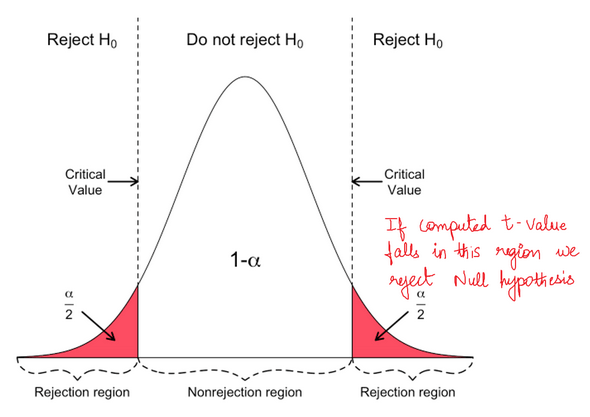
\includegraphics[width=0.7\textwidth]{figures/stats/one_side_t_test_rejection_regions.png}
\caption{
Illustration of a two-tail $t$-test's null hypothesis, $H_{0}$ rejection regions,
by \href{https://www.machinelearningplus.com/statistics/t-test-students-understanding-the-math-and-how-it-works/}{Selva Prabhakaran}.
In a one-tail $t$-test we would only consider the tail on a single side.
$\alpha$ is the significance level, typically \num{0.05} or lower.
}
\label{fig:two_sided_t_test}
\end{figure}

%%%%%%%%%%%%%%%%%%%%%%%%%%%%%%%%%%%%%%%%%%%%%%%%%%%%%%%%
\subsection{One-Sample}
\label{stats:t_test:one}
In a one-sample $t$-test we have one sample of size $n$ with mean $\expval{x}$ and standard deviation $s$,
and test the null hypothesis that it belongs to a parent population with mean $\mu_{0}$.
In this case the parent population does not need to be normally distributed, but the distribution of possible $\expval{x}$ is assumed to be normal.

The $t$-statistic \cref{eq:stats:t:one} can be used with $\nu = n-1$ to find a $\pvalue$.

\begin{equation}\label{eq:stats:t:one}
t = \frac{\expval{x} - \mu_{0}}{s / \sqrt{n}}
\end{equation}

%%%%%%%%%%%%%%%%%%%%%%%%%%%%%%%%%%%%%%%%%%%%%%%%%%%%%%%%
\subsection{Two-Sample: Unpaired}
\label{stats:t_test:two:unpaired}
In a two-sample unpaired $t$-test we have two independent samples, each of size $n$,
but with their own sample means $\expval{x_{i}}$ and standard deviations $s_{i}$.
Provided that we can assume that the two parent distributions of $x_{1}$ and $x_{2}$ have the same variance,
we can test the null hypothesis that the two parent distribution means are equal.

The $t$-statistic \cref{eq:stats:t:two:unpaired} can be used with $\nu = 2n-2$ to find a $\pvalue$.

\begin{subequations}\label{eq:stats:t:two:unpaired}
\begin{align}
t &= \frac{\expval{x_{1}} - \expval{x_{2}}}{s_{p} \sqrt{2/n}} \label{eq:stats:t:two:unpaired:t} \\
s_{p} &= \sqrt{\left(s^{2}_{x_{1}} + s^{2}_{x_{2}}\right)/2} \label{eq:stats:t:two:unpaired:s_p}
\end{align}
\end{subequations}

%%%%%%%%%%%%%%%%%%%%%%%%%%%%%%%%%%%%%%%%%%%%%%%%%%%%%%%%
\subsubsection{Different Sample Sizes}
\label{stats:t_test:two:unpaired:diff_n}
If we relax the sample size condition and let $n_{1} \neq n_{2}$
we can still compute a $t$-statistic,
provided the parent distribution's variances are equal\footnote{A useful rule of thumb is $1/2 < s_{x_{1}} / s_{x_{2}} < 2$.}.

The $t$-statistic \cref{eq:stats:t:two:unpaired:diff_n} can be used with $\nu = n_{1} + n_{2} - 2$ to find a $\pvalue$.

\begin{subequations}\label{eq:stats:t:two:unpaired:diff_n}
\begin{align}
t &= \frac{\expval{x_{1}} - \expval{x_{2}}}{s_{p} \sqrt{\frac{1}{n_{1}} + \frac{1}{n_{2}}}} \label{eq:stats:t:two:unpaired:diff_n:t} \\
s_{p} &= \sqrt{\left(\left(n_{1} - 1\right)s^{2}_{x_{1}} + \left(n_{2} - 1\right)s^{2}_{x_{2}}\right)/\left(n_{1} + n_{2} -2\right)} \label{eq:stats:t:two:unpaired:diff_n:s_p}
\end{align}
\end{subequations}

%%%%%%%%%%%%%%%%%%%%%%%%%%%%%%%%%%%%%%%%%%%%%%%%%%%%%%%%
\subsubsection{Different Sample Sizes and Variances (Welch's \texorpdfstring{$t$}{t}-test)}
\label{stats:t_test:two:unpaired:diff_n_diff_var}
If we further relax the assumptions and also let the population variances differ
we arrive at Welch's $t$-test which approximates\footnote{The
true distribution of $t$ depends somewhat on the unknown population variances,
see the \href{https://en.wikipedia.org/wiki/Behrens\%E2\%80\%93Fisher_problem}{Behrens--Fisher problem}
for more.} the $t$-distribution.

The $t$-statistic \cref{eq:stats:t:two:unpaired:diff_n_diff_var:t} can be used with $\nu$ \cref{eq:stats:t:two:unpaired:diff_n_diff_var:dof} to find a $\pvalue$.

\begin{subequations}\label{eq:stats:t:two:unpaired:diff_n_diff_var}
\begin{align}
t &= \frac{\expval{x_{1}} - \expval{x_{2}}}{\sqrt{\frac{s^{2}_{1}}{n_{1}} + \frac{s^{2}_{2}}{n_{2}}}} \label{eq:stats:t:two:unpaired:diff_n_diff_var:t} \\
\nu &= \frac{\left(s^{2}_{1}/n_{1} + s^{2}_{2}/n_{2}\right)^{2}}{\frac{\left(s^{2}_{1}/n_{1}\right)^{2}}{n_{1}-1} + \frac{\left(s^{2}_{2}/n_{2}\right)^{2}}{n_{2}-1}} \label{eq:stats:t:two:unpaired:diff_n_diff_var:dof}
\end{align}
\end{subequations}

%%%%%%%%%%%%%%%%%%%%%%%%%%%%%%%%%%%%%%%%%%%%%%%%%%%%%%%%
\subsection{Two-Sample: Paired}
\label{stats:t_test:two:paired}
In a two-sample paired $t$-test we have two dependent samples,
such as two sets of measurements from the same $n$ individuals taken at different times.
In this case, we are testing the null hypothesis that the difference in means of the two dependent samples is $\mu_{0}$.
Note, we can set $\mu_{0} = 0$ if we simply want to test for a statistically significant difference, and not an \apriori degree of difference.
Defining the difference between paired observations as $x_{\Delta}$, we compute the mean difference $\expval{x_{\Delta}}$ and $s_{\Delta}$ standard deviation on the sample.

The $t$-statistic \cref{eq:stats:t:two:paired} can be used with $\nu = n-1$ to find a $\pvalue$.

\begin{equation}\label{eq:stats:t:two:paired}
t = \frac{\expval{x_{\Delta}} - \mu_{0}}{s_{\Delta} / \sqrt{n}}
\end{equation}

%%%%%%%%%%%%%%%%%%%%%%%%%%%%%%%%%%%%%%%%%%%%%%%%%%%%%%%%
%%%%%%%%%%%%%%%%%%%%%%%%%%%%%%%%%%%%%%%%%%%%%%%%%%%%%%%%
\section{\texorpdfstring{$\chi^{2}$-Test}{Chi-Squared Test}}
\label{stats:chi2_test}

Pearson's $\chi^{2}$-test can be used to
statistically compare a set of observations in
$n$ variables, $x_{i}$, to prior expectations via the $\chi^{2}$-distribution.
The \pvalue returned by the test estimates the probability of obtaining the observations
assuming the null hypothesis, \ie the expectations, is true.
The $\chi^{2}$-test statistic, $X^{2}$, is created with the assumption that
the data are normally distributed and independent,
which often is the case due to the central limit theorem.
It is constructed by squaring the difference\footnote{Yates's
correction for continuity $\left(x^{\text{obs}}_{j} - x^{\text{exp}}_{j}\right)^{2} \to \left(\abs{x^{\text{obs}}_{j} - x^{\text{exp}}_{j}}-0.5\right)^{2}$ may
also be applied in some low statistics cases.} between
an expected value, $x^{\text{exp}}_{i}$, and its corresponding observation, $x^{\text{obs}}_{i}$,
and dividing by the expectation:

\begin{equation}\label{eq:stats:chi2_score}
X^{2} = \sum_{i=1}^{n} \frac{\left(x^{\text{obs}}_{i} - x^{\text{exp}}_{i}\right)^{2}}{x^{\text{exp}}_{i}}\,.
\end{equation}

In the limit that each $x^{\text{obs}}_{i}$ is normally distributed and $n$ is large, $X^{2} \to \chi^{2}$.
We can then use the $\chi^{2}$ distribution with $\nu = n-1$ degrees of freedom to find the \pvalue as the area to the right of $X^{2}$.
An easy way to compute $X^{2}$ and the \pvalue is to use the \texttt{scipy.stats.chisquare(f\_obs, f\_exp)}
\href{https://docs.scipy.org/doc/scipy/reference/generated/scipy.stats.chisquare.html}{function}.

The $\chi^{2}$-test can also be used to test of the data's independence, or homogeneity,
for $m$ samples of $n$ variables with $\nu = \left(n-1\right)\left(m-1\right)$ and\footnote{Note this is really the same as \cref{eq:stats:chi2_score} if we reindex, just with a different $\nu$.}

\begin{equation}\label{eq:stats:chi2_score_ind}
X^{2} = \sum_{i=1}^{n} \sum_{j=1}^{m} \frac{\left(x^{\text{obs}}_{i,j} - x^{\text{exp}}_{i,j}\right)^{2}}{x^{\text{exp}}_{i,j}}\,.
\end{equation}

%%%%%%%%%%%%%%%%%%%%%%%%%%%%%%%%%%%%%%%%%%%%%%%%%%%%%%%%
%%%%%%%%%%%%%%%%%%%%%%%%%%%%%%%%%%%%%%%%%%%%%%%%%%%%%%%%
\section{Binomial Proportion Test}
\label{stats:binomial_test}
When dealing with samples of $n$ binary events we can perform hypothesis testing
on the number of observed positive events $k$
using test statistics built on the binomial distribution.

%%%%%%%%%%%%%%%%%%%%%%%%%%%%%%%%%%%%%%%%%%%%%%%%%%%%%%%%
\subsection{Exact Binomial Test}
\label{stats:binomial_test:exact}
For small $n$ it is possible to compute the \pvalue
explicitly from the binomial distribution \cref{eq:stats:binomial}.
We test the null hypothesis that the probability of success is $\pi_{0}$
having actually observed $k$ successes, $k = n \pi$.

The \pvalue is then the sum

\begin{equation}\label{eq:stats:binomial_test:exact}
\pvalue = \sum_{i \in \, \mathcal{I}} {n \choose i}\pi_{0}^{i} \left(1-\pi_{0}\right)^{n-i},
\end{equation}

\noindent where $\mathcal{I}$ depends on the type of test:

\begin{table}[H]
\centering
\begin{tabular}{l|l}
$\pi < \pi_{0}$ & $\mathcal{I} = \left\{0, 1, \ldots, k\right\}$, \\
$\pi > \pi_{0}$ & $\mathcal{I} = \left\{k, k+1, \ldots, n\right\}$, \\
$\pi \neq \pi_{0}$ & $\mathcal{I} = \left\{\forall \, i: P\left(x=i\right) \leq P\left(x = k\right)\right\}$, with binomial $P\left(x\right)$ \cref{eq:stats:binomial}.
\end{tabular}
\end{table}

%%%%%%%%%%%%%%%%%%%%%%%%%%%%%%%%%%%%%%%%%%%%%%%%%%%%%%%%
\subsection{One-Sample}
\label{stats:binomial_test:one}
For large sample sizes the binomial distribution is approximated by the normal distribution
and we can use a form of the $Z$-test to produce {\pvalue}s.
We require the observations to be independent,
\ie we may only sample $< \SI{10}{\percent}$ of the parent population,
the sampling distribution of $\pi$ to be approximately normal,
and that there are $\geq 10$ successes and $\geq 10$ failures,
$n \pi_{0} \geq 10$ and $n \left(1-\pi_{0}\right) \geq 10$, \ie the success-failure condition.

The $Z$-score is then:

\begin{equation}\label{eq:stats:binomial_test:one}
Z = \frac{\pi - \pi_{0}}{\sqrt{\pi_{0}\left(1-\pi_{0}\right)/n}} = \frac{k - n \pi_{0}}{\sqrt{n\pi_{0}\left(1-\pi_{0}\right)}}.
\end{equation}

Note that the one-sample test is provided by the
\texttt{scipy.stats.binomtest} \href{https://docs.scipy.org/doc/scipy/reference/generated/scipy.stats.binomtest.html}{function}.

%%%%%%%%%%%%%%%%%%%%%%%%%%%%%%%%%%%%%%%%%%%%%%%%%%%%%%%%
\subsection{Two-Sample}
\label{stats:binomial_test:two}
In the case of two samples, we can test the null hypothesis
that the difference\footnote{Again, we set $\pi_{\Delta} = 0$ if we want to test for any difference.} in the sample's probabilities is $\pi_{\Delta}$.
We require that the $\pi$ from the two samples are uncorrelated,
have approximately normal sampling distributions,
and that their difference $\pi_{1} - \pi_{2}$ is an unbiased estimator.

The $Z$-score is then:

\begin{subequations}\label{eq:stats:binomial_test:two}
\begin{align}
Z &= \frac{\pi_{1} - \pi_{2} - \pi_{\Delta}}{\pi_{p} \left(1-\pi_{p}\right)\left(1/n_{1} + 1/n_{2}\right)} \label{eq:stats:binomial_test:two:Z} \\
\pi_{p} &= \frac{k_{1} + k_{2}}{n_{1} + n_{2}} \label{eq:stats:binomial_test:two:pi_p}
\end{align}
\end{subequations}

%%%%%%%%%%%%%%%%%%%%%%%%%%%%%%%%%%%%%%%%%%%%%%%%%%%%%%%%
%%%%%%%%%%%%%%%%%%%%%%%%%%%%%%%%%%%%%%%%%%%%%%%%%%%%%%%%
\section{Hypothesis Test Power}
\label{stats:power}
% TODO

%%%%%%%%%%%%%%%%%%%%%%%%%%%%%%%%%%%%%%%%%%%%%%%%%%%%%%%%
%%%%%%%%%%%%%%%%%%%%%%%%%%%%%%%%%%%%%%%%%%%%%%%%%%%%%%%%
\section{Maximum Likelihood Estimation (MLE)}
\label{stats:MLE}
% TODO

% TODO under ``regularity assumptions'', MLE converges to the true optimal values as $n \to \infty$, is usually biased but bias is reduced as $n \to \infty$, efficient - variance approximates Cramer-Rao lower bound for larger samples

%%%%%%%%%%%%%%%%%%%%%%%%%%%%%%%%%%%%%%%%%%%%%%%%%%%%%%%%
%%%%%%%%%%%%%%%%%%%%%%%%%%%%%%%%%%%%%%%%%%%%%%%%%%%%%%%%
\section{Maximum A Posteriori (MAP)}
\label{stats:MAP}
% TODO In maximum \aposteriori (MAP) estimation
